
%----------------------------------------------------------------------------------------
%	CHAP introduction
%----------------------------------------------------------------------------------------

\chapterimage{blue-chapter-head_4-reduced.pdf} % Chapter heading image

\chapter{Introduction}\label{chap:Introduction}
\section{Background}
The MetaR software \url{http://MetaR.campagnelab.org} is an example of a new kind of interactive tool for data analysis. It was developed by the Campagne laboratory using the Meta Programming System (MPS) (see \url{http://www.jetbrains.com/mps}~\cite{Dmitriev:2004}. MPS is a mature Language Workbench that makes it relatively easy to create new languages and tools to help users of these languages~\cite{campagne2014mps}. 

\section{Intended audience}
This booklet is designed to teach how to use MetaR for data analysis. In the first chapters, we will assume that you have no prior scripting or programming experience, but will expect you to know how to use a computer.

%TODO re-enable the next sentence when the chapters have been written:
%Chapters~\ref{chap:Intentions}and~\ref{chap:ExtendingMetaR} will be useful for users who also have programming experience. These chapters explain how such users can extend MetaR with intentions or new language constructs.

\section{Key Concepts}
\paragraph{High-level data abstractions}
MetaR is designed to make it easier to conduct data analysis. To achieve this goal, and in contrast to programming languages such as the R language, Julia or Python, that are often low-level and require good programming skills, MetaR offers high-level data abstractions and provides assistance in manipulating data. High-level abstractions used in MetaR analyses include the following concepts:

\begin{enumerate}
	\item Tables, Columns, Column Groups and Group usages,
	\item Analyses
	\item Plot
	\item Model
\end{enumerate}

\noindent{}These high-level abstractions will be explained in the following chapters.

\paragraph{R program generation}
Analyses developed with MetaR are transformed into R programs when the user needs to execute them. MetaR is tightly integrated with MPS to make it seamless to run analyses without prior knowledge of the R language.
\begin{remark}
Note that while most users can use MetaR without knowledge of the R language, all users will need to install the R language in order to execute MetaR analyses.
\end{remark}

\paragraph{Docker integration}

Starting with version 1.3.1, MetaR can run the R scripts that it generates into Docker containers. Docker is a technology that makes it easier to obtain reproducible script executions. When MetaR does not use Docker, it is possible for the R runtime to try to install a package the first time you run an analysis with a statement that requires the package. While this should not be a problem, we found that R package installation is brittle and can sometimes fail at various time points, for a variety of reasons\footnote{For instance, because a new version of a package has become available which breaks compilation of the package on your machine.}. To avoid such problems, which tend to occur when we give a training sessions, we now support running Analyses with Docker. Chapter~\ref{chap:DockerIntegration} explains how to configure MetaR to use Docker for reproducible analyses.
\mbox{}
\begin{flushright}

\includegraphics[width=1.5in]{figures/DockerImage.png}
\end{flushright}
\paragraph{Composable language}
MetaR is built as an MPS language. In contrast to languages built with compiler technology, MPS languages are composable. Briefly, language composition is the ability to compose, or combine, two or more languages. This ability is particularly useful to extend MetaR. It is possible to define micro-languages, made of one or two statement types, that when composed with MetaR make it possible to customize MetaR for specific application domains. The EdgeR language provides an example of composition, where an R/Bioconductor package called EdgeR has been integrated with MetaR and exposes a new kind of statement to perform calls of differential expression. See Chapter~\ref{chap:EdgeR} to learn more about language composition in MetaR.
  
\section{Solutions and Models}
Developing an analysis with MetaR is done by creating nodes of the MetaR concepts in MPS models. Models exist in MPS solutions. To learn how to create an MPS solution, read the preview of the MPS language workbench available at \url{http://campagnelab.org/publications/our-books/}\cite{campagne2014mps}, or watch the beginning of the MetaR training video at \url{http://campagnelab.org/software/metar/video-tutorials/}. Figures~\ref{fig:QuickStartMenu}-\ref{fig:NewProjectDialog} provide a brief walk-through of the steps you should follow to create a project and solution. After the project open, open the project tab(see ~\cite{campagne2014mps}) and right-click on the solution name. Import the metaR devkit and create a model. 

You can create as many models as you need to store your analyses. In the following chapter, we assume that you have created a solution and at least one model in this solution. 


\begin{SCfigure}
  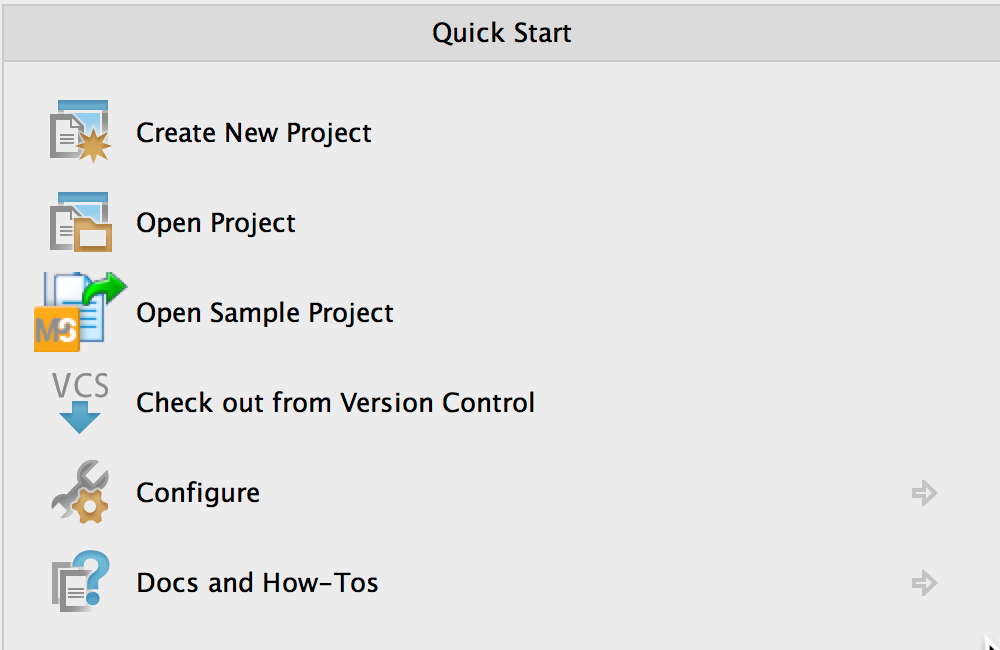
\includegraphics[width=\figWidthNarrow]{figures/QuickStart.png}
  \caption[The Quick Start menu.]{\textbf{The Quick Start menu.} This menu is displayed when you first open MPS, or when you have no project currently open in MPS. The first item in the menu is used to create a new project. 
}\label{fig:QuickStartMenu}
\end{SCfigure}

\begin{SCfigure}
  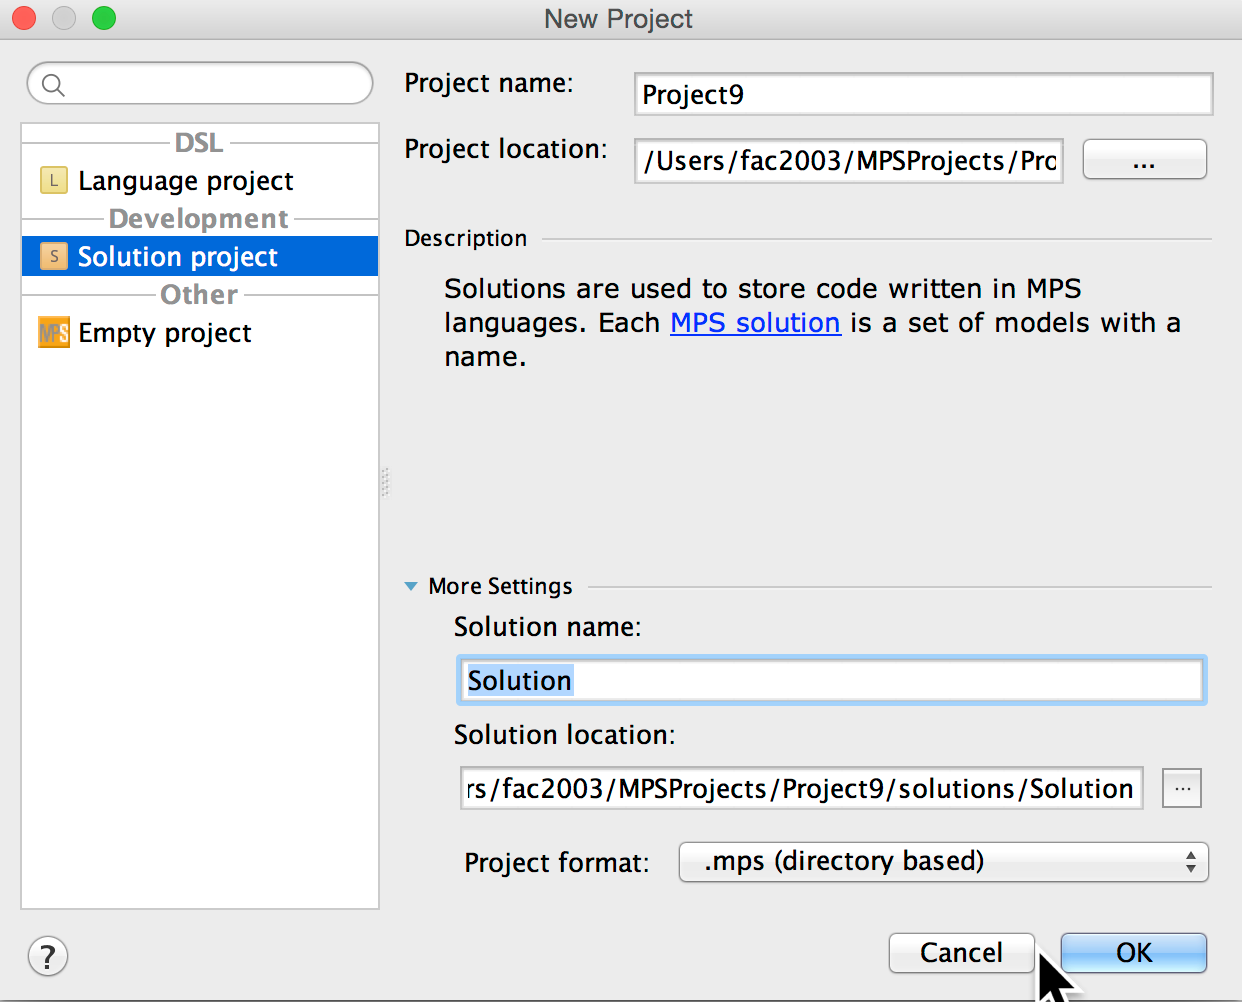
\includegraphics[width=\figWidthNarrow]{figures/NewSolutionWizard.png}
  \caption[The New Project Dialog.]{\textbf{The New Project Dialog.} Use this dialog to create a new Solution. Solutions are used to store models and express your solutions to specific analysis problems. Select the ``Solution Project'' project type on the left panel, name the project, and name the solution you wish to create.
}\label{fig:NewProjectDialog}
\end{SCfigure}
